\documentclass{article}
\usepackage{tikz}
\usetikzlibrary{shapes.geometric, arrows.meta}

\tikzset{
  block/.style = {rectangle, draw=black, fill=white, text centered, rounded corners, minimum width=3cm, minimum height=1cm},
  line/.style = {->, thick, >=stealth}
}

\begin{document}

\begin{figure}[h]
\centering
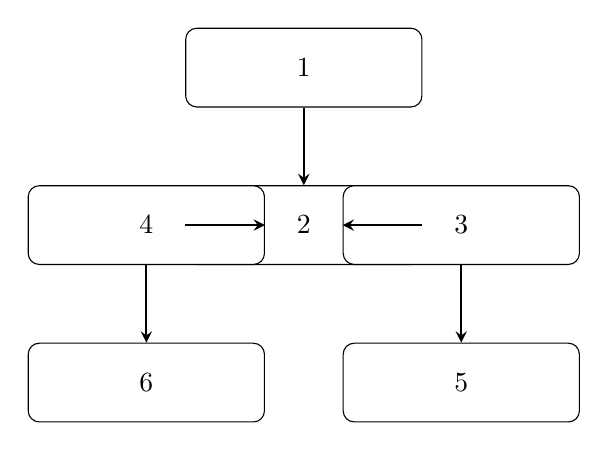
\begin{tikzpicture}[node distance=2cm]

% Nodes
\node (A) [block] {1};
\node (B) [block, below of=A] {2};
\node (C) [block, right of=B] {3};
\node (D) [block, left of=B] {4};
\node (E) [block, below of=C] {5};
\node (F) [block, below of=D] {6};

% Lines
\draw [line] (A) -- (B);
\draw [line] (B) -- (C);
\draw [line] (B) -- (D);
\draw [line] (C) -- (E);
\draw [line] (D) -- (F);

\end{tikzpicture}
\caption{Hasse Diagram for Björner's Example}
\label{fig:bjorner-example}
\end{figure}

\end{document}